% Reviewed input SHA256 d8b3a6090148f1ea7d3d49c20bb01d2349b345e5c1fab5d0c209021fb0f17e4e benchmark/protocols/mechanism-windows-pilot-v1.json
% Reviewed input SHA256 c99b15bf200d78d57b25faf668de37d7fb0c04cfd9c2729640fb6798859f1772 benchmark/analysis/outputs/windows-followup-intake-v1/comparison-summary.json
% Reviewed input SHA256 8b89658b151fa4a0852038f497e6838edaf18da3409b56b7f199b86827f87a37 benchmark/analysis/outputs/windows-followup-intake-v1/numpy-summary.json
% Reviewed input SHA256 d4b9ce12c23ecdbff615bc6566e2a5a61e43cf073aeadbb7f193bd82db670f86 benchmark/analysis/outputs/windows-followup-intake-v1/runtime/SUMMARY.json
% Reviewed input SHA256 1d3576fe927db1433c2712f5caaff45c24aacaf6401527068754323feeda0ffa manuscript/software/intake.generated.tex
% Reviewed input SHA256 749f6f6710211b9cde823f13f051db57e45ad6b9a1c59d5cb3f9766b9f449f9e manuscript/software/followup.template.tex
% Reviewed input SHA256 cb5bc9c51a9735d5e7f7a10de697c141ecac47093c26c6de5d505042a7b29329 figures/windows-mechanism-pilot-v1/work-and-cached-cost.pdf
% Reviewed input SHA256 04d86adde990daa6809994ed97b0cbd3fb81a940771a5f0e6a54101b02134c7f benchmark/analysis/outputs/mechanism-windows-pilot-v1/windows-20261006/analysis-cpu/workflows.csv
% Reviewed input SHA256 9e2fd3b87f61bbb453aac19b038c42bbe11710d5d2ff455239b5ffafe48c4b8b benchmark/analysis/outputs/mechanism-windows-pilot-v1/windows-20261006/analysis-cuda/workflows.csv
% Input SHA256 c34ec98f0093c93effb5a37fbaeb8c8739b1d7f5ad263825e3272317a047eaec benchmark/analysis/outputs/windows-round2-intake-v1/summary.json
第二轮接收把无约束路径、参数变换与下游诊断分别核对。
108份MH保存路径均在原容差内，接受事件失配为0；但从同一无约束状态在Mac重算原尺度输出时，
60份不满足原逐位相等要求，最大绝对差为$8.88\times10^{-15}$。
这项严格跨系统检查仍记为失败，不能通过事后添加容差改称全部通过。
Windows同机核验与Mac跨系统重算回答不同问题。

CPU Pyro NUTS在9个目标上的串行/四进程技术对照中，54组保存数组逐字节相同。
对收到的18份原二进制重新计算R诊断，有限$\hat R$与tail ESS一致，
bulk ESS最大差约$1.02\times10^{-12}$，不可判定位置一致。
这不意味着重复计算后验函数也必然逐位相同，更不增加独立统计重复数。
原短链的探索不足仍然成立。

实际数组传递同样是复现契约的一部分。第二轮启动时，Windows重新生成的六份候选输入中，噪声与导数探测数组相同，但对数均匀数组有82/49152个元素不同，最大差约$4.44\times10^{-16}$，因此原协议拒绝启动机制工作流。随后传递原始封存文件，按原哈希和容差完成了下述测量；原启动失败与候选数组仍保留。相同种子和依赖版本不能替代实际数组校验，核验本身也未确定底层数学库差异的因果来源。

\subsection{Windows有限机制测量}
独立机制协议在G1、G2、L1上各使用2份主随机输入，比较窗口4/16、链数分配及预先规定的G2 RWM步长对照。CPU与CUDA各完成96个工作流；每个工作流包括首次审计、3次交错缓存重放和探针后重放。全部960份保存路径通过独立NumPy参考核验，接受事件零失配，最大绝对路径差为$3.84\times10^{-10}$。技术重放、窗口变体和跨设备副本均不增加独立输入数。

测量使用同一台Windows 11计算机的Ryzen 7 9800X3D和RTX 5080，torch主机线程设为4，CUDA使用float64并显式同步。桌面显示负载仍存在，不将线程数等同独占物理核心数。表\ref{tab:windows-mechanism}给出全部配置的描述性比值；它们来自三次缓存sample时间中位数之比，既不是完整推断成本比，也不是跨独立重复的置信区间。

\begin{table}[htbp]\centering\small
\begin{tabular}{lrrl}\toprule
设备/执行器 & 配对数 & 比值大于1 & 全部比值范围\\\midrule
CPU / quasi-DEER & 24 & 0 & 0.092--0.322 \\
CPU / Picard & 36 & 20 & 0.612--3.574 \\
CUDA / quasi-DEER & 24 & 0 & 0.139--0.437 \\
CUDA / Picard & 36 & 32 & 0.778--4.805 \\
\bottomrule\end{tabular}
\caption{机制协议的同核缓存执行比值：同组顺序时间除以时间执行器时间。全部120个时间执行配置均保留；quasi-DEER对应MALA，Picard对应RWM。每模型仅两份独立输入，配对数不能解释为独立实验数。}
\label{tab:windows-mechanism}
\end{table}

quasi-DEER每个输出转移对应7.75--22.5次前向映射及3.875--11.25次JVP；Picard为2--7.59375次前向映射（图\ref{fig:windows-mechanism}）。这些计数包括拒绝自环，均高于顺序执行的一次前向映射；映射与JVP不是等价浮点工作量，不能简单相加。每端6个工作流完全零接受，全部保留。例如G2/RWM步长1.0的第一份输入，在窗口4/16下可一次确认整个窗口，同时没有接受移动。因此较长的确认前缀可以由自环产生，并不表示更有效的后验探索。

\begin{figure}[htbp]\centering
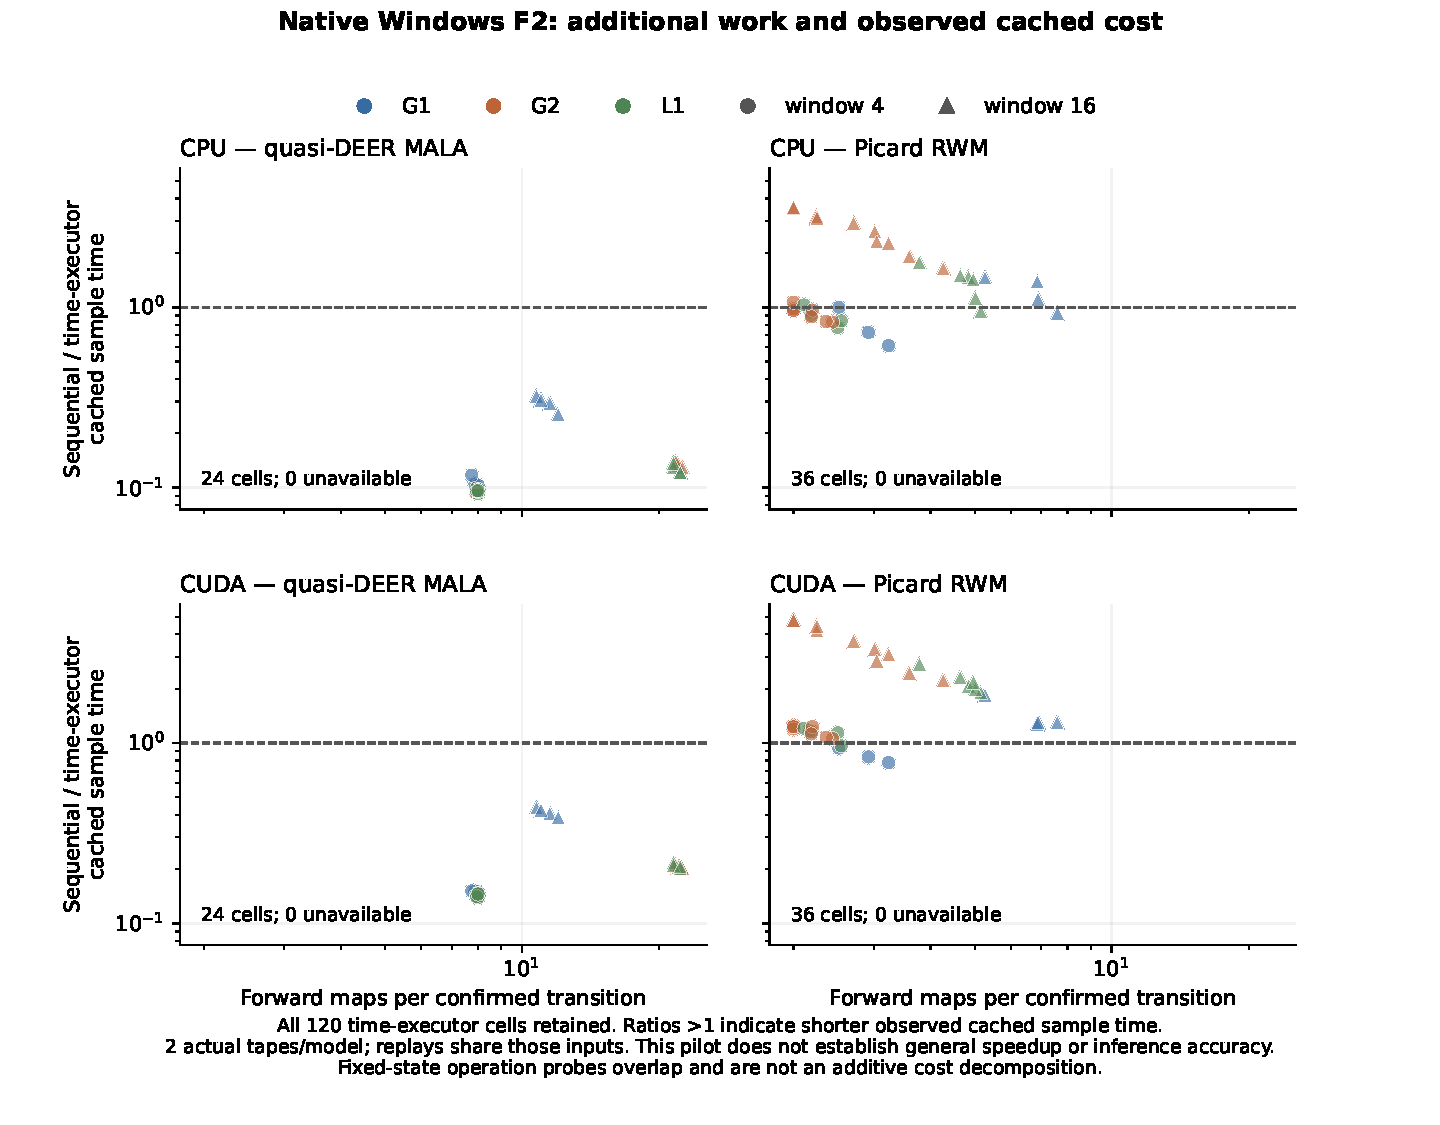
\includegraphics[width=\linewidth]{../../figures/windows-mechanism-pilot-v1/work-and-cached-cost.pdf}
\caption{Windows机制测量中的重复求值与缓存成本。每点为一个配置与实际输入的组合，共120点，部分重叠；颜色区分目标，点形区分窗口。上下行为CPU/CUDA，左右列为quasi-DEER/Picard。纵轴大于1表示指定缓存执行较短；横轴包括拒绝自环。三次技术重放不扩充独立样本量，图中没有推断精度或统计区间。操作探针存在重叠，不用于构造可加的独占耗时分解。}
\label{fig:windows-mechanism}
\end{figure}

预先规定的等512个总输出对照提供了另一种解释边界。在G2、L1的两份输入及两个设备上，16条各32步的顺序链均比单条512步、窗口16的Picard链更快，后者时间为前者的4.43--6.92倍。这8个技术对照说明链数分配会改变执行吞吐；两种分配的轨迹长度、初始化份数及探索能力不同，不能解释为相同推断精度下的优劣。图示的额外工作量与quasi-DEER减速相容，但不足以唯一归因于JVP、扫描或主机控制；固定状态操作探针与生产路径不同，同步及嵌套操作也使各阶段不能相加还原总时间。

\subsection{批次运行与安装的实测范围}
另一个Windows技术批次完成27项主任务和24项缓存探测（96次调用），包含最大形状、进程集合管理和终态恢复检查。接收端对保存MH数组独立重放，并核对函数与R诊断；这没有新增正式推断重复。90条函数诊断中仍有59条$\hat R>1.01$及27条tail ESS不可判定，不能将运行成功解释为收敛。该批次支持其封存运行器的技术能力；后续正式协议适配器的独立Windows验收与充分预算比较仍需完成。

Python 0.2.0.dev2与R 0.2.0.9002候选已在Windows新建依赖环境和仓库外完成安装核验，覆盖CPU/CUDA MH和R批量入口。默认R包检查与显式集成测试分别保存；成功检查不隐去此前安装和locale失败。接收端核对源码、sdist、wheel与R包中17个模块，并从保存RDS重建诊断，没有在Mac重新测量CUDA。该证据不涵盖原生Windows的JAX/Stan安装、GPU NUTS或第三方团队的独立复现。
